\documentclass[crop,tikz,convert={outext=.svg,command=\unexpanded{pdf2svg \infile\space\outfile}},multi=false]{standalone}
\usetikzlibrary{decorations.pathreplacing}

% Color to white
\makeatletter
\newcommand{\globalcolor}[1]{%
  \color{#1}\global\let\default@color\current@color
}
\makeatother
\AtBeginDocument{\globalcolor{white}}

\begin{document}
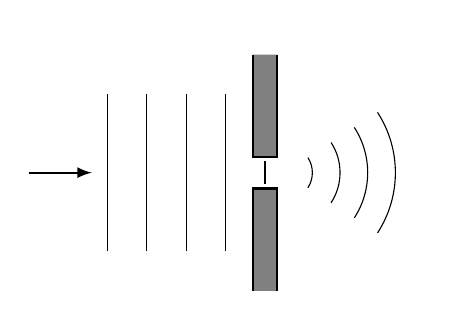
\begin{tikzpicture}[slit/.pic={%
\draw[thick,fill=gray] (-0.15,1.5) |- (0.15,0.2) -- (0.15,1.5)
(-0.15,-1.5) |- (0.15,-0.2) -- (0.15,-1.5);
\draw (0,0.15) -- (0,-0.15);
\node[anchor=south,font=\sffamily\bfseries] at (0,1.6){#1};},
decoration={expanding waves,angle=33}]

 \begin{scope}
  \pic (0,0) {slit};
  \foreach\X in {-2,-1.5,-1,-.5} 
  {\draw(\X,-1)--(\X,1);}
  \draw[thick,-latex] (-3,0) -- (-2.2,0);
  \draw[decorate] (0.25,0) -- (2,0);
 \end{scope}
 %
\end{tikzpicture}
\end{document}
